\documentclass{article}
\usepackage{amssymb}
\usepackage{authblk}
\usepackage{caption}
\usepackage{color}
\usepackage{float}
\usepackage[margin=0.8in]{geometry} % FIXME: Choose sensible
\usepackage{graphicx}
\usepackage[utf8]{inputenc}
\usepackage{listings}
\usepackage{natbib}
%\usepackage[style=authoryear,backend=biber]{biblatex}

% FIXME: This is for automatic sizing of nested parentheses
%\usepackage{nath}
%\delimgrowth=1

\usepackage{nth}
\usepackage{soul}

% Big-O notation 
%\newcommand{\BigO}[1]{\ensuremath{\operatorname{O}\left(#1\right)}} % FIXME
%\newcommand{\BigO}[1]{\ensuremath{\operatorname{O}\bigl(#1\bigr)}}
%\newcommand{\bigO}[1]{\ensuremath{\mathop{}\mathopen{}\mathcal{O}\mathopen{}\left(#1\right)

\begin{document}

\title{CSCI435 Project}
\author{Paul Foster
	\thanks{Email: \texttt{pf981@uowmail.edu.au}}
	\thanks{Student Number: \texttt{3648370}}}
\affil{University of Wollongong}
\date{2013 Spring}

\maketitle

\renewcommand\abstractname{Executive Summary}
\begin{abstract}
This report evaluates various computer vision technologies for the Gwynville Airport Authority's security and surveillance system. Haar cascade classifiers were used to detect faces of a photo of students and several face recognition algorithms (Eigenfaces, Fisherfaces, Local Binary Patterns (LBP) and Local Intensity Distribution (LID)) where applied to individual photos of students. The results indicate that Haar cascade classifiers are effective in real-time accurate face detection and would be ideal for a people-counting surveillance system. After testing several face-recognition algorithms it finds that LBP provides efficient and accurate results that are less sensitive to variance in pose. The report recommends that the Haar cascade classifiers should be used to count passengers and then the faces obtain from that should be used with LBP to determine identities. These identities can be used to update "Frequent Users" cards and also be used to add to the LBP training data.
\end{abstract}

\section{Introduction}
Face detection and face recognition are two actively-researched and important topics in computer vision. Both of these tasks are performed frequently and easily by humans however no current automated system exists that can be deployed effectively in an unconstrained setting \cite{sinha2006face}.

Earlier forms of facial recognition involved holistic methods such as Eigenfaces\cite{turk1991eigenfaces} and Fisherfaces\cite{belhumeur1997eigenfaces}. However, more recently, local descriptors such as Local Binary Patterns (LBP)\cite{ahonen2004face} and Local Intensity Distribution (LID)\cite{nguyen2011local} have gained attention due to their efficiency and tolerance to pose and illumination changes.

Face recognition technology has significantly progressed since the proposal of the Eigenface method in 1987. Given that most individuals can only identify a few thousand people, under constrained conditions (such as fixed facial expression and lighting) and a very large number of classifications, automated face recognition can perform better than human recognition \cite{li2011handbook}.

However, facial recognition is not possible if the face is not isolated from the background \cite{wilson2006facial} which is why face detection is so important. Various face detection algorithms exist which have their own strengths and weaknesses. Skin detection algorithms are used to detect skin based on colour and shape but have problems discriminating between faces and other parts of skin whereas Haar-like feature detection uses a pattern classification approach.

There are numerous commercial and law-enforcement applications for face detection and recognition including advanced video surveillance, user authentication and suspect tracking \cite{zhao2003face}. The effectiveness of these applications rely on the efficiency and accuracy of the underlying algorithms. This report will compare the efficiency and accuracy of 4 facial recognition algorithms: Eigenfaces, Fisherfaces, Local Binary Patterns (LBP) and Local Intensity Distributions (LID). We will also investigate the efficiency and performance of Haar feature-based cascade classification for face detection and discuss how these algorithms can be applied by the Gwynville Airport Authority for their security and surveillance system.



\section{People Counting Algorithms}
\subsection{Data Preparation}
To reduce computation, images were uniformly scaled such that their area was approximately 480*600.

\subsection{Haar Cascade Classifiers for Face Detection}
Haar classifiers can be used to rapidly detect faces within an image in real time. Haar-like features use the contrast variances between groups of pixels to determine relative light and dark areas. Two or three adjacent groups form a Haar-like feature. This can be applied to objects of different sizes by scaling the features.

Haar cascade classifiers combine several weak detectors where each weak detector is a simple binary classifier. Each weak detector forms a cascade stage.
If an image patch passes through all the cascade stages, it is classified as "positive". Otherwise it is discarded.

\subsubsection{Detecting Features}
%http://www.cognotics.com/opencv/servo_2007_series/part_2/sidebar.html
Let $A_I[x,y]$ denote the integral image of image $A[x,y]$. We define the integral image as the array containing the sums of pixel's intensities directly left or above a pixel, $(x, y)$. That is,
\begin{equation}
	A_I[x,y] = \sum_{x^\prime\le x, y^\prime\le y}A(x^\prime, y^\prime)
\end{equation}

In a similar way, we can calculate the rotated integral image, $A_R[x,y]$, as the sum of pixel intensities located forty five degrees to the left and above the x value and below the y value. That is,
\begin{equation}
	A_R[x,y] = \sum_{x^\prime\le x, x^\prime\le x-|y-y^\prime|}A(x^\prime, y^\prime)
\end{equation}

Features are detected by taking the appropriate integral image and the difference between six to eight array elements to form two or three connected rectangles.

Figure~\ref{fig:features} shows some simple features.
\begin{figure}[H]
\centering
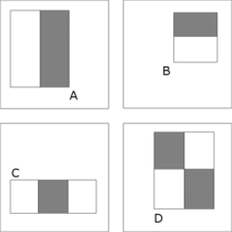
\includegraphics[width=0.2\linewidth]{./haarfeatures}
\caption{Basic Haar-like features}
\label{fig:features}
\end{figure} % FIXME

\subsubsection{AdaBoost}
AdaBoost is an algorithm for constructing a strong classifier, $f(x)$, as a linear combination of weak classifiers, $h_t(x)$. That is, $f(x)=\sum_{t=1}^{T}\alpha_th_t(x)$. It is used to both select the best features and to train the classifiers that use them.

It achieves this using the following algorithm.\\

\noindent Given $(x_1, y_1),\ldots,(x_m,y_m)$ where $x_i\in X, y_i\in\{-1,+1\}$, initialise $D_1(i)=1/m$ for $i=1,\ldots,m$.

\noindent For $t=1,\ldots,T$:

We choose a weak classifier $h_t$ such that $h_t = argmax_{h_t\in H}|0.5 - \epsilon_t$ where $\epsilon_t = \sum_{i=1}^m D_t(i)I(y_i\ne h_t(x_i))$ where $I$ is the indicator function.

If $|0.5 - \epsilon_t| \le \theta$. Where $\theta$ is some threshold, then stop.

Choose $\alpha_t=\frac{1}{2}ln(\frac{1-\epsilon_t}{\epsilon_t})$.

For $i=1,\ldots,m$: update $D_{t+1}(i)=\frac{D_t(i)exmp(\alpha(2I(y_i\ne h_t(x_i))-1))}{\beta}$. Where $\beta$ ensures $D_{t+1}$ will be a probability distribution.

The final classifier is $H(x)=sign(\sum_{t=1}^T\alpha_th_t(x))$.



\subsubsection{Training}
The Haar cascade classifier is trained with hundreds of samples of faces, called positive examples. Each of these samples are scaled to the same size. Negative examples are arbitrary images of the same size. From this training, we get many weak classifiers.

AdaBoost is used to create cascade the weak classifiers arranged in order of complexity.

\subsubsection{Detecting faces}
To find faces in an image, the image is scanned by looking at different regions of interest across the image, each region of interest is decided to either contain a face or not based on whether or not it passes through each of the cascade stages. If an image patch passes through all the cascade stages, it is classified as "positive". Otherwise it is discarded.

This is computationally efficient as most non-faces will be discarded in the earlier stages of the cascade meaning that the complex subsequent cascade stages do not need to be computed.

\subsubsection{Parameter Optimisation}
OpenCV provides several trained XML files for face detection with Haar. The results showed that haarcascade\_frontalface\_alt2.xml provided the best results, as others such as haarcascade\_frontalface\_default.xml failed to detect some of the faces. The XML file was generated via a tree-based 20*20 gentle adaboost frontal face detector.

There were four parameters to consider with the Haar cascade classifier: \textbf{double} $scaleFactor$, \textbf{int} $minNeighbors$, \textbf{Size} $minSize$ and \textbf{Size} $maxSize$.

It was found that more faces were detected (either correctly or as false positives) as $scaleFactor$ was increased and $minNeighbors$ was decreased.

Starting at $minNeighbors$=3, the value was incrementally increased until a sufficient amount of noise (false positives) was removed. The value was maximised such that it still detected every face in the image. This resulted in minimising false positives.

Similarly for $scaleFactor$, starting at 1.005, the value was increased until every face was detected and there were no false positives.

$minSize$ and $maxSize$ were left unspecified as this would allow for detection of people at significantly varying distances to the camera.

The final parameters chosen were $scaleFactor$=0.01 and $minNeighbors$=9.

\subsubsection{Face Detection Results}
After the parameters were optimised, all faces were successfully detected almost instantly. This can be seen in figure~\ref{fig:group}.
\begin{figure}[H]
\centering
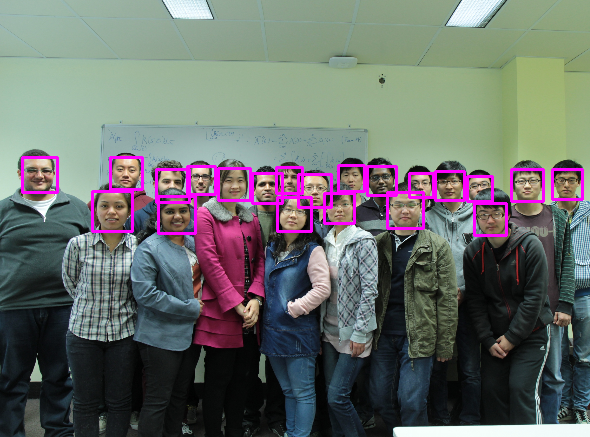
\includegraphics[width=0.7\linewidth]{./groupdetected}
\caption{Faces detected. $scaleFactor=1.01, minNeighbors=9$}
\label{fig:group}
\end{figure}

The results support the notion that Haar cascade classifiers are suitable for real-time detection of faces.

\section{Face Recognition Algorithms}
\subsection{Data Preparation}
The individual face data given consisted of between 9 and 14 photos each of the faces of 11 students. The images were converted to grayscale then were scaled down and cropped to 128*128. This was achieved by uniformly scaling the image such that the smaller dimension was equal to 128 pixels. The 128*128 rectangle centred at the centre of the image was then used as the cropped image. 128*128 was chosen because it was large enough to provide good results but not so large as to be computationally problematic.

For group photos, where we wanted to use the face-counting algorithm, the photo was uniformly scaled such that its area was approximately 640*480 to reduce computation.

\subsubsection{Training/Testing Split}
\label{sec:split}
The student photos were split into two sets: a training set and a validation set. They were used to train the classification model and measure the performance of the model respectively. There can be no overlap in these two sets as trained images will obviously be classified correctly and will not give accurate real-world performance measures.

The proportion of the size of the training set to the size of the validation set was chosen to be 7:3. The choice of this ratio is a balance between better classification with more training data, or more accurate performance estimates with more test data.

70\% of the data were used to train the model and the other 40\% were used to test its performance.

\subsection{Eigenfaces}
If we describe the collection of all images of the face of an individual as a vector space, then we can describe every such image through a linear combination of the spanning vectors of that space.

The goal is to find the principal components of the training data, called eigenfaces. These eigenfaces form a basis for every image of this person’s face. That is, every image of this person’s face can be described as a linear combination of the eigenfaces. Furthermore, every image of this person’s face can be approximated by a linear combination of the eigenfaces with the largest eigenvalues.

\subsubsection{Calculating Eigenfaces}
Given $M$ training images with dimensions $h$*$w$, we consider each image as an $D$-dimensional vector where $D = hw$.

\vspace{12pt} \noindent Let $S$ be the set of the $M$ training images.
\begin{equation}
	S = \left\{\Gamma_1, \Gamma_2, \Gamma_3, \ldots, \Gamma_M\right\}
\end{equation}
Let $\Psi$ denote the average face of $S$. That is,
\begin{equation}
	\Psi = \frac{1}{M}\cdot\sum_{n=1}^{M}\Gamma_n
\end{equation}
Let $\Phi_i$ denote the difference between the $i$\textsuperscript{th} training face and the average.
\begin{equation}
	\Phi_i = \Gamma_i - \Psi
\end{equation}
Constructing the covariance matrix, $C \in \mathbb{R}^{D\times D}$, we get
\begin{equation}
	C = \frac{1}{M}\cdot\sum_{n=1}^{M}\Phi_n \Phi_n^T
	  = AA^T
\end{equation}
Where $A = [\Phi_1 \Phi_2 \ldots \Phi_M]$

We wish to calculate the eigenvectors ($u_1, \ldots, u_s$) of $C$. However, solving this directly is typically a computationally infeasible task.

Instead, consider the eigenvectors, $v_i$ of $A^TA$ such that $A^TAv_i=\widehat{\lambda}_iv_i$. Premultiplying by $A$ yields $AA^TAv_i=\widehat{\lambda}_iAv_i$. So clearly, $Av_i$ are the eigenvectors of $C=AA^T$.

We construct $L \in \mathbb{R}^{M\times M}$ as $L = A^T A$ such that $L_{mn} = \Phi^T_m \Phi_n$ and find the $M$ eigenvectors ($v_1, \ldots, v_k$) of $L$. These are used to computer the eigenfaces
\begin{equation}
	u_l = \sum_{k=1}^{M}v_{lk}\Phi_k \qquad k=1, \ldots, M
\end{equation}
Using this method reduces the computation from $\mathcal{O}(D)$ to $\mathcal{O}(M)$ where $M\ll D$.

To reduce the dimensionality, we keep only the eigenvectors with the largest corresponding eigenvalue. These vectors account for the most variation in the images.

\subsubsection{Using Eigenfaces for Face Recognition}
To classify a face image $\Gamma$, we project it into its "face space" using $\omega_k = u^T_k(\Gamma - \Psi)$, for $k = 1, \ldots, M^\prime$.

Let $\Omega^T = [\omega_1, \ldots, \omega_{M^\prime}]$ and let $\Omega_k$ denote the vector describing the $k$th face class.

We wish to find $k$ that minimises $\epsilon_k = \|(\Omega - \Omega_k)\|$. If such an $\epsilon_k$ is above some threshold $\theta_\epsilon$, then we say the face is unknown. Otherwise we classify the face as the $k$th class.

\subsubsection{Parameter Optimisation}
There were two parameters to consider with Eigenfaces: \textbf{int} $numComponents$, \textbf{double} $threshold$. $numComponents$ determines how many dimensions to keep when we reduce dimensionality and $threshold$ is our $\theta_\epsilon$ defined in the previous section.

It was found that reducing $numComponents$ reduced the performance of the algorithm, however it also resulted in reduced $\epsilon_k$. A problem was encountered where we either had reasonable performance, but $\epsilon_k$ was in the thousands, or we had poor performance with small $\epsilon_k$. There seemed no value for $numComponents$ that had no downside. A value of 80 was chosen as it was sufficiently high for reasonable performance, however the distances ($\epsilon_k$) were still very large.

As stated previously, our $\epsilon_k$ distances were extremely large so our $threshold$ had to be very large too. As one would expect, reducing this number increased the number of $unknown$ classifications which could potentially reduce the number of false classifications. $threshold$ was chosen to be one of the smaller misclassified $\epsilon_k$'s. This was 4710.0 (which is extremely large).

\subsection{Fisherfaces}
The main advantage of this method is that it is invariant to different light sources. Extensive experimental results show that Fisherface has lower error rates than eigenface on the havard and yale face detection databases \cite{belhumeur1997eigenfaces}.

The Fisherfaces method recognises that variance among faces in the database may come from distortions such as illumination changes or facial expressions. Sometimes these variations within a face class are larger than the variations between classes of faces.

Like Eigenfaces, the Fisherfaces algorithm reduces the dimensionality of the problem. It does so in a way the preserves the linear separability of the classes. We wish to choose basis vectors, $W$, such that the ratio of the between-class scatter and within-class scatter is maximised. We define the between-class scatter matrix as $S_B = \sum_{i=1}^{c}N_i(\mu_i - \mu)(\mu_i - \mu)^T$ and the within-class scatter matrix as  $S_W = \sum_{i=1}^{c}\sum_{x_k\in X_i}(x_k - \mu_i)(x_k - \mu_i)^T$. Where $u_i$ is the mean image of class $X_i$ and $N_i$ is the number of samples in class $X_i$.

$S_W$ is either singular or non-singular. If it is singular, choose $W_{opt}$ as the matrix with orthonormal columns such that $\frac{|W^TS_BW|}{|W^TS_WW|}$ is maximised. That is
\begin{equation}
	W_{opt} = arg\ max_W \frac{|W^TS_BW|}{|W^TS_WW|} = [w_1\ w_2\ \ldots\ w_m]
\end{equation}
Where $w_i$ is the $i$th generalised eigenvector of $S_B$ and $S_W$ corresponding to the $m$ largest generalised eigenvalues ($\lambda_1, \ldots, \lambda_m$). So we have
\begin{equation}
	S_Bw_i = \lambda_iS_Ww_i,\quad i=1, \ldots, m
\end{equation}
However, in face recognition problems, $S_W$ is always singular \cite{belhumeur1997eigenfaces}. To solve this problem, we use PCA to project the image to a lower dimensional space such that $S_W$ is nonsingular. We wish to find $W_{opt}^T$ such that $W_{opt}^T = W_{fld}^TW_{pca}^T$ where $W_{pca} = arg\ max_W|W^TS_TW|$ and $W_{fld} = arg\ max_W\frac{|W^TW_{pca}^TS_BW_{pca}W|}{|W^TW_{pca}^TS_WW_{pca}W|}$.
%FIXME: IS THIS DONE???
\subsubsection{Parameter Optimisation}
There were two parameters to consider with Fisherfaces: \textbf{int} $numComponents$, \textbf{double} $threshold$.

It was found that reducing $numComponents$ reduced the performance of the algorithm, however it also resulted in reduced distances between the face and the face class. A problem was encountered where we either had reasonable performance, but the distance was in the thousands, or we had poor performance with small distance. $numComponents$ was chosen such that it maximised the performance which was found to be the number of classes minus 1.

As stated previously, our distances were extremely large so our $threshold$ had to be very large too. As one would expect, reducing this number increased the number of $unknown$ classifications which could potentially reduce the number of false classifications. $threshold$ was chosen to be one of the smaller misclassified distances. This was 1500 (which is extremely large).

\subsection{Local Binary Patterns}
The LBP descriptor describes a pixel as an $P$-bit binary number based on the values of $P$ points on the circumference of a circle of radius $R$ centred at the pixel. This number becomes its label.

Because LBP converts pixels to an binary number, computations can be done with integer arithmetic which results in significant performance advantages over the other methods which use floating-point arithmetic.

We will define a uniform pattern to be a binary pattern containing at most two bitwise transitions from 0 to 1 or 1 to 0 when the pattern is traversed circularly. For example $01110000$ and $00000000$ are uniform whereas $01101000$ and $00110011$ are not.

Let $(P, R)$ denote the pixel neighbourhood of $P$ evenly-spaced points on the circumference of a circle of radius $R$.

Let $LBP^{u^2}_{P,R}\cdot$ denote the LBP operator in a $(P, R)$ neighborhood using only uniform patterns ($u^2$) and labelling all remaining patterns with a single label.
% FIXME: http://www.scholarpedia.org/article/Local_Binary_Patterns

The LBP operator works by comparing the pixel to each of its $P$ neighbours. Where the centre pixel's value is greater than the neighbour's value, write "1". Otherwise, write "0". This results in a $P$-bit binary number.

\begin{figure}[H]
\centering
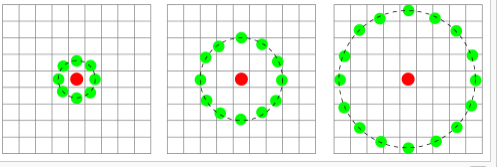
\includegraphics[width=0.4\linewidth]{./lbp}
\caption{LBP Neighbours}
\label{fig:lbp}
\end{figure}

\subsubsection{Training LBP}
Training involves obtaining a description for each training image.

Each of the training images are trained in the following way. Each pixel, $p$, is given a classification of $LBP_{P,R}^{u^2}(p)$. The image is split evenly into $X$ columns and $Y$ rows and the histogram of the local binary patterns of its constituent pixels is determined. These histograms are then normalised.

Our description for the image consists of a spacial histogram: $X\cdot Y$ histograms, which each correspond to a region of the image, appended together.

\subsubsection{Face Recognition Using LBP}
Given an unclassified image $I$, its description (a spacial histogram) is determined using the previous method. For each of the training images $I^{(i)}$, the chi-squared distance between the training image's spacial histogram, $H^{(i)}$, and the unclassified image's histogram, $H$, is calculated.
We classify the image as the class of the closest training image. That is,
\begin{equation}
	class\{I\} = class\{I^{(k)}\}
\end{equation}
where $I_k$'s spacial histogram has the smallest chi-squared distance to $I$'s spacial histogram. That is, $k$ is chosen such that
\begin{equation}
	\chi^2(H, H^{(k)}) = \sum_{j=1}^{n}\frac{(H_j - H^{(k)}_j)^2}{H_j + H^{(k)}_j}
\end{equation}
is minimised, where $H^{(k)}_j$ denotes the $j$th element of the spacial histogram $H^{(k)}$.

We add the additional constraint that $class\{I\}$ will be \textit{unknown} if the distance is not within some threshold, $\theta$. That is,
\begin{equation}
	\chi^2(H, H^{(i)}) > \theta \Rightarrow class\{I\} = unknown
\end{equation}

\subsubsection{Additional Notes}
Many enhancements have been proposed for LBP. These include considering neighbours that lie on an ellipse rather than a circle, non-rectangular regions, weighted regions, regions of different sizes and overlapping regions \cite{belhumeur1997eigenfaces}. However, we will only be testing the method specified above.


\subsubsection{Parameter Optimisation}
With LBP, there were 5 parameters that we needed to optimise: \textbf{int} $radius$, \textbf{int} $neighbors$, \textbf{int} $gridX$, \textbf{int} $gridY$, \textbf{double} $threshold$.

$radius$ refers to the radius of the circle we consider our neighbours to lie on whereas $neighbors$ refers to the number of neighbours. Increasing $radius$ tended to reduce performance, even when $neighbors$ was scaled appropriately. $radius=1$ and $neighbors=8$ tended to give the best results.

The grid parameters refer to how many regions we want to break the image up into. Whilst varying $gridX$ and $gridY$ significantly affected performance, it was erratic and there was no way to predict this trend. It was found that $gridX=7$ and $gridY=7$ gave good performance.

$threshold$ was chosen to be one of the smaller misclassified distances, which was $52$.

\subsection{Local Intensity Distribution}
Local Intensity Distribution (LID) descriptors can be used to describe the features of an intensity image by capturing the distribution of local intensity differences. Similar to LBP descriptors, LID descriptors are insensitive to illumination changes.

\subsubsection{The LID Descriptor}
Let $I(x,y) : \mathbb{Z}^2 \rightarrow \mathbb{R}$ denote the intensity image of an image/patch with $N$ pixels and let $p = (x,y) \in \mathbb{Z}^2$ be an arbitrary point in the domain of $I$. We define $LID_{N,R}(p) : \mathbb{Z}^2 \rightarrow \mathbb{R}^N$ as
\begin{equation}
   % \label{simple_equation}
   LID_{N,R}(p) = \langle d(p_1,p), \ldots, d(p_n,p)\rangle
\end{equation}
where $d(p_i,p) = I(p_i) - I(p)$ (quantised uniformly into $M$ levels) and $p_i = (x_i, y_i) \in \mathbb{Z}$ is such that $max\{|x_i - x|, |y_i - y|\} = R$.
For all $p_i$ in the patch, we calculate $ LID_{N,R}(p_i)$.
We determine the probability density function of $v=\{v_1,\ldots,v_N\}$ over the entire patch and call it $u(v)$ where $d(p_i,p)$ is a realisation of $v_i$. $u(v)$ is the LID descriptor for the patch $I$.
%We group together the first elements of all $LID_{N,R}(p)$ for each point into a normalised histogram and call it $u_1$. We group together the second elements of all $LID_{N,R}(p)$ for each point into a normalised histogram and call it $u_2$. We do the same for all elements of $LID_{N,R}$ to get $u=(u_1,\ldots,u_N)$ where $u_i$ is a normalised histogram representing the probability distribution of the $d(p_i,p)$ for all $p$ in the patch. $u$ is our LID descriptor for the patch.

\subsubsection{Training The Images}
We wish to train a codebook, $C=\{c_1, \ldots, c_N\}$, where $c_i$ is an equalised histogram representing the $i$th training image and each $c_i$ has a label associated with it.

$c_i$ is calculated in the following way. A set of keypoints, $\{k_1, \ldots, k_n\}$, are generated using SIFT detector on the $i$th image training image. The LID descriptor for the $(2L+1)\times(2L+1)$ region centred at each of these keypoints are calculated.

The descriptors are then clustered using a K-means algorithm using the chi-squared distance measure.

We store the resulting centroids as they will be needed for the face recognition stage.

The results of the K-means algorithm are used to generate a histogram with $K$ bins. We equalise this histogram to get $c_i$. The label associated with $c_i$ is the class of the $i$th training image.

\subsubsection{Face Recognition Using LID}
Given an unclassified image, $I$, we extract its SIFT keypoints and calculate the LID descriptors for the $(2L+1)\times(2L+1)$ region centred at each of these keypoints.

Using the centroids from the training stage, we cluster the descriptors in a similar manner to the training stage.

The results are used to generate a histogram which is then normalised and call it $c$. We classify the image as the class of the closest training image. That is $class\{I\}=class\{I_k\}$ where $k$ is such that $c_k$ of the codebook has smallest chi-squared distance to $c$. That is, we choose $k$ such that
\begin{equation}
	\chi^2(c, c_k) = \sum_{j=1}^{n}\frac{(c^{(j)} - c^{(j)}_k)^2}{c^{(j)} + c^{(j)}_k}
\end{equation}
is minimised, where $c^{(j)}_k$ denotes the $j$th element of the histogram $c_k$.

We add the additional constraint that $class\{I\}$ will be \textit{unknown} if the distance is not within some threshold, $\theta$. That is,
\begin{equation}
	\chi^2(c, c_k) > \theta \Rightarrow class\{I\} = unknown
\end{equation}

\subsubsection{Alternative Methods for LID Face Detection}
\label{sec:alternativeLID}
For our LID algorithm, we use the chi-squared measure of distance, however the original paper on LID uses the Kullback-Leiber (KL) distance \cite{nguyen2011local}. It is unlikely that this will cause any differences in terms of performance, however the KL distance may have a computational advantage.
% FIXME: I suspect that if you use spacial histograms instead of SIFT you will get better results

\subsection{Results}
The results involved testing the 89 images of the validation set. For how this set was constructed, see Section~\ref{sec:split}.
\begin{table}[H]
	\centering
    \begin{tabular}{|l|l|}
    \hline
    Algorithm & Failure Rate (\%) \\
    \hline
    Eigenfaces & 40.45\% \\
    Fisherfaces & 32.58\% \\
    LBP & 11.25\% \\
    LID & 94.38\% \\
    \hline
    \end{tabular}
    \caption {Failure rates for face detection algorithms}
\end{table}

Clearly, LID's performance is unexpected. This is discussed in~\ref{sec:lidbad}.

In terms of efficiency, as expected LBP was both the quickest to train and detect as it uses integer arithmetic rather than floating point. LID was the next most efficient with Eigenfaces and Fisherfaces being the least efficient.


\subsubsection{Why Eigenfaces and Fisherfaces Performed Worse Than Expected}
The Eigenfaces and Fisherfaces methods have been reported to have a 4\%\cite{turk1991eigenfaces} and 4.6\%\cite{belhumeur1997eigenfaces} failure rate respectively, however our testing showed only 40.45\% and 32.58\% respectively. The reason for this discrepancy is likely because both of these methods are sensitive to pose \cite{turk1991eigenfaces}\cite{belhumeur1997eigenfaces}. The reported good performance of these methods have been on databases which contained faces with only one frontal view. The images we have tested with in this report have had very varying poses (See figure~\ref{fig:pose}). This may be the cause of these algorithms poor performance.

\begin{figure}[H]
\centering
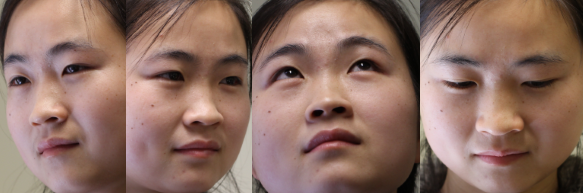
\includegraphics[width=0.7\linewidth]{./pose}
\caption{Images showing variation in pose in the dataset}
\label{fig:pose}
\end{figure} % FIXME

Although the Eigenfaces and Fisherfaces implementations used in this report are sensitive to variance of pose, there exist modern modifications to these algorithms to reduce that sensitivity \cite{jaiswal2012local}.

\subsubsection{Why The LID Implementation Performed so Poorly}
\label{sec:lidbad}
Overall, the LID algorithm for face recognition performed very poorly. Of the four algorithms it by far performed the worst in terms of correctly identifying faces. This is likely due to implementation issues rather than issues with the underlying algorithm.

\subsection{Comparison}
Both Eigenfaces and Fisherfaces performed poorly with failure rates of 40.45\% and 32.58\% respectively. These two algorithms were the least efficient both in training and in detection.

The results show that LBP was by far the most accurate with an 11.25\% failure rate. It was also the most efficient with both training and detection which is like attributable to its use of integer arithmetic rather than floating point.

Unfortunately, we are unable to meaningfully interpret LID's results. (See section~\ref{sec:lidbad}).

Eigenfaces and Fisherfaces are both sensitive to variance in pose. Fisherfaces is less sensitive than Eigenfaces to variance in pose, and lighting, which may explain its better performance. LBP is less sensitive to variance in pose and lighting to Fisherfaces, which may explain its performance.

\section{Conclusion}
From the results of the people-counting experiments, we can conclude that Haar cascade classifiers are suitable for real-time, accurate face detection.

From the results of our face recognition experiments, we can conclude that LBP by far performed the best and was the most efficient.

However, it should be noted that the images were all taken in the same room, with the same lighting so these results are not necessarily indicative of performance under different conditions.

\section{Recommendation}
From the results of this report, we can conclude that Haar cascade classifiers provide a suitable real-time people-counting algorithm for the Gwynville Airport Authority's  people-counting surveillance system.

After testing several face-recognition algorithms, the results indicate that LBP provides efficient and accurate results that are less sensitive to variance in pose.

The report recommends that the Haar cascade classifiers should be used to count passengers and then the faces obtain from that should be used with LBP to determine identities. These identities can be used to update "Frequent Users" cards.

In addition to this, the new faces can be added to the training data to continually train the LBP. If the face is unrecognised, a class will be added. If the face is recognised, the face will be added to the training data with the appropriate class.

\bibliographystyle{plain}
\bibliography{references}




\end{document}
% FIXME: There is a problem: The page numbers restart in the middle Just hack it to work - they only want the pdf :-( Don't know why
% FIXME: For training, we don't really test false positives. We could give it some faces not in the dataset.
% FIXME: Look at http://people.wku.edu/qi.li/teaching/595_BA/ba16_Eigenface.pdf for cross-validation in determining the best split
% If you run out of space: http://www.terminally-incoherent.com/blog/2007/09/19/latex-squeezing-the-vertical-white-space/
% You could talk about the evolution of LBP - originally just 8 neighbors then circle then ellipse. Originally didn't exclude non-uniform binary patterns. The regions do not have to be rectangular or the same size and do not have to cover the whole image - could even overlap.
% THIS IS A REALLY GOOD LBP PAPER - might illuminate some info for LID: http://web.ing.puc.cl/~asoto/papers/Maturana-09.pdf
%Eigen failures: 40.4494%
%Fisher failures: 32.5843%
%LBP failures: 11.236%
%LID failures: 94.382%
%http://stackoverflow.com/questions/5808434/how-does-the-viola-jones-face-recognition-method-work